\chapter{Redundancy Reduction: Barlow Twins and VICReg}
\label{ch:barlow_twins}

% 1. Descriptive Opening
In the landscape of self-supervised learning, the dominant paradigm for extracting meaningful representations from unlabeled data has long been contrastive learning. As explored in previous chapters, methods like InfoNCE and SimCLR operate by pulling together representations of augmented views of the same image (positive pairs) while pushing apart representations of different images (negative pairs). The repulsive force between negative pairs is crucial; without it, the neural network would succumb to \emph{representation collapse}, mapping all inputs to a single, trivial constant vector to perfectly minimize the distance between positive pairs. 

However, relying on negative pairs introduces significant computational and statistical burdens. Contrastive methods require enormous batch sizes or large memory banks to ensure that the negative samples adequately cover the data manifold. If the batch size is too small, the repulsive force is insufficient to prevent partial collapse or dimensional redundancy, where multiple features encode the exact same underlying factor of variation. 

To circumvent this, researchers returned to a foundational idea from neuroscience: \emph{redundancy reduction}. In 1961, the neuroscientist Horace Barlow proposed that the goal of sensory processing in the brain is to recode highly correlated sensory inputs into a format that minimizes statistical dependencies between neurons. By decorrelating the neural firing patterns, the brain maximizes the information capacity of its representation, ensuring that each neuron codes for a statistically independent feature of the environment.

When imported into deep learning, redundancy reduction provides an elegant solution to representation collapse that completely bypasses the need for negative pairs. Instead of comparing sample embeddings in a batch against other sample embeddings (a sample-centric approach), redundancy reduction compares the \emph{features} against other \emph{features} across the batch (a feature-centric approach). If two feature dimensions are highly correlated across a batch of images, one of them is redundant. By penalizing the cross-correlation between different feature dimensions, the network is forced to utilize its entire representational capacity, naturally avoiding collapse without ever needing to explicitly push samples apart.

This chapter delves into the mathematical formulations of two seminal methods that instantiate this principle: Barlow Twins and VICReg (Variance-Invariance-Covariance Regularization). We will explore how their objective functions map directly onto information-theoretic quantities, proving how forcing feature decorrelation acts as a tractable surrogate for maximizing the entropy and mutual information of deep representations.

% 2. Mathematical Core
\section{The Barlow Twins Objective}

Let $\mathcal{D}$ be a dataset of images drawn from $P_{\text{data}}$. For a given batch of size $B$, let $X \in \mathbb{R}^{B \times C \times H \times W}$ represent the input batch. We apply two stochastic data augmentations $T, T' \sim \mathcal{T}$ to yield twin views $X^A = T(X)$ and $X^B = T'(X)$. A deep neural network $f_\theta$ processes these views to produce $d$-dimensional embeddings $Z^A = f_\theta(X^A)$ and $Z^B = f_\theta(X^B)$, where $Z^A, Z^B \in \mathbb{R}^{B \times d}$.

In the Barlow Twins framework, the representations are first mean-centered and standardized along the batch dimension for each feature $i \in \{1, \dots, d\}$:
\begin{align}
    \tilde{z}^A_{b,i} &= \frac{z^A_{b,i} - \mu^A_i}{\sigma^A_i}, \quad \mu^A_i = \frac{1}{B}\sum_{b=1}^B z^A_{b,i}, \quad \sigma^A_i = \sqrt{\frac{1}{B}\sum_{b=1}^B (z^A_{b,i} - \mu^A_i)^2 + \epsilon}
\end{align}
A symmetric normalization is applied to $Z^B$ to yield $\tilde{Z}^B$. The empirical cross-correlation matrix $\mathcal{C} \in \mathbb{R}^{d \times d}$ is computed as:
\begin{equation}
    \mathcal{C}_{i,j} = \frac{1}{B} \sum_{b=1}^B \tilde{z}^A_{b,i} \tilde{z}^B_{b,j}
\end{equation}
Note that $\mathcal{C}_{i,j} \in [-1, 1]$. The Barlow Twins loss function is defined as:
\begin{equation}
    \mathcal{L}_{\text{BT}} = \underbrace{\sum_{i=1}^d (1 - \mathcal{C}_{i,i})^2}_{\text{Invariance}} + \lambda \underbrace{\sum_{i=1}^d \sum_{j \neq i} \mathcal{C}_{i,j}^2}_{\text{Redundancy Reduction}}
\end{equation}
where $\lambda > 0$ is a trade-off hyperparameter. The \emph{invariance} term forces the diagonal elements of $\mathcal{C}$ to 1, meaning the embedding of a feature should be identical across augmented views. The \emph{redundancy reduction} term forces all off-diagonal elements to 0, ensuring that different feature dimensions are decorrelated.

\begin{figure}[ht]
\centering
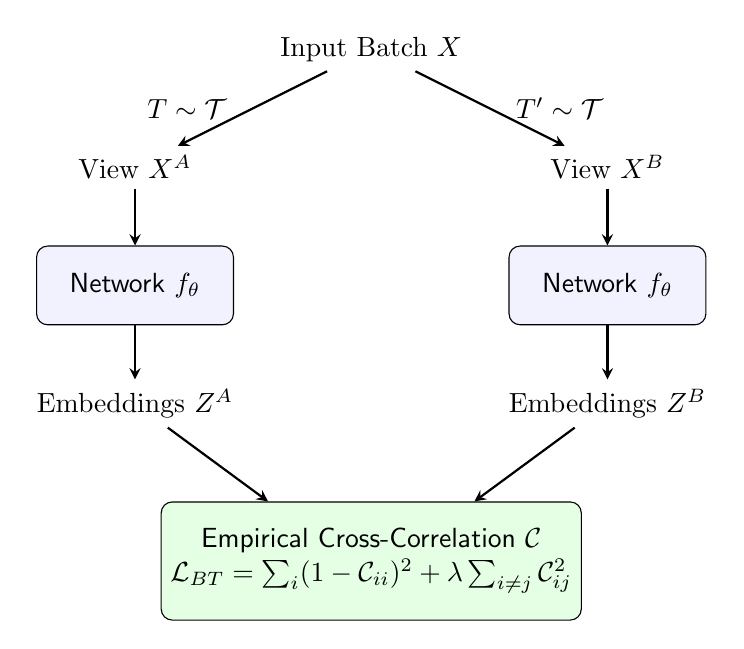
\begin{tikzpicture}[
    box/.style={draw, rectangle, minimum width=2.5cm, minimum height=1cm, fill=blue!5, font=\sffamily, rounded corners},
    arrow/.style={->, thick, >=stealth}
]
\node (x) at (0, 0) {Input Batch $X$};
\node (xa) at (-3, -1.5) {View $X^A$};
\node (xb) at (3, -1.5) {View $X^B$};
\node[box] (fa) at (-3, -3) {Network $f_\theta$};
\node[box] (fb) at (3, -3) {Network $f_\theta$};
\node (za) at (-3, -4.5) {Embeddings $Z^A$};
\node (zb) at (3, -4.5) {Embeddings $Z^B$};
\node[box, fill=green!10, minimum width=5cm, minimum height=1.5cm, align=center] (loss) at (0, -6.5) {Empirical Cross-Correlation $\mathcal{C}$ \\ $\mathcal{L}_{\text{BT}} = \sum_i (1-\mathcal{C}_{ii})^2 + \lambda \sum_{i \neq j} \mathcal{C}_{ij}^2$};

\draw[arrow] (x) -- (xa) node[midway, left=2mm] {$T \sim \mathcal{T}$};
\draw[arrow] (x) -- (xb) node[midway, right=2mm] {$T' \sim \mathcal{T}$};
\draw[arrow] (xa) -- (fa);
\draw[arrow] (xb) -- (fb);
\draw[arrow] (fa) -- (za);
\draw[arrow] (fb) -- (zb);
\draw[arrow] (za) -- (loss.150);
\draw[arrow] (zb) -- (loss.30);
\end{tikzpicture}
\caption{The Barlow Twins architecture. Instead of contrasting individual samples, the objective forces the cross-correlation matrix of the batch features to approximate the identity matrix.}
\label{fig:bt_arch}
\end{figure}

\section{Information-Theoretic Equivalence}

The intuitive mechanism of Barlow Twins maps formally to maximizing mutual information. Contrastive methods maximize $I(X^A; Z^B)$ using bounds like InfoNCE. Redundancy reduction methods achieve the same end by decomposing the mutual information.

\begin{theorem}[Barlow Twins and Information Maximization]
Assume that the embeddings $Z^A$ and $Z^B$ are jointly Gaussian vectors in $\mathbb{R}^d$. Minimizing the Barlow Twins loss $\mathcal{L}_{\text{BT}}$ serves as a surrogate for maximizing the mutual information $I(Z^A; Z^B)$ under the constraint of feature decorrelation.
\end{theorem}
\begin{proof}
Recall the mutual information can be written as:
\begin{equation}
    I(Z^A; Z^B) = H(Z^A) - H(Z^A | Z^B)
\end{equation}
For a $d$-dimensional multivariate Gaussian $Z \sim \mathcal{N}(\mu, \Sigma)$, the differential entropy is $h(Z) = \frac{1}{2} \log \det(2\pi e \Sigma)$.
To maximize $H(Z^A)$, we wish to maximize $\det(\Sigma^A)$. Because the Barlow Twins framework standardizes the variance of each feature (so the trace of $\Sigma^A$ is fixed to $d$), Hadamard's inequality states that $\det(\Sigma^A) \leq \prod_{i=1}^d \Sigma^A_{ii} = 1$, with equality occurring if and only if $\Sigma^A$ is a diagonal matrix.
Thus, by penalizing the off-diagonal elements of the cross-correlation matrix (and implicitly the auto-correlation matrix), the redundancy reduction term $\sum_{i \neq j} \mathcal{C}_{ij}^2$ pushes the covariance structure toward the identity matrix, effectively maximizing the marginal entropy $H(Z^A)$ and $H(Z^B)$ within the constrained space.

Conversely, the conditional entropy $H(Z^A | Z^B)$ measures the uncertainty in $Z^A$ given $Z^B$. By driving the diagonal elements $\mathcal{C}_{ii}$ to 1, the invariance term forces $Z^A$ to be perfectly predictable from $Z^B$ for each dimension, thereby minimizing $H(Z^A | Z^B)$.
Consequently, combining these terms maximizes $I(Z^A; Z^B)$ without necessitating negative samples.
\end{proof}

\begin{figure}[ht]
\centering
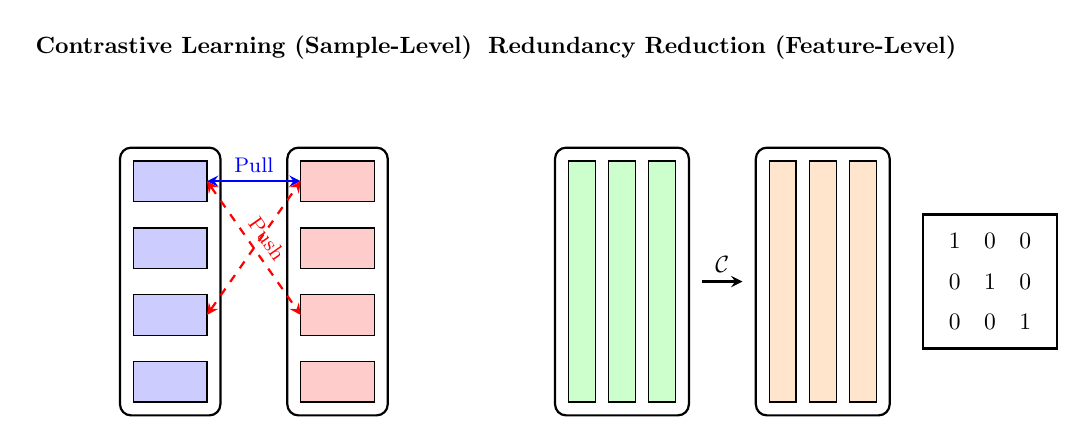
\begin{tikzpicture}[scale=0.85, transform shape, >=stealth]
% Contrastive
\node[align=center, font=\bfseries] at (2, 5.5) {Contrastive Learning   (Sample-Level)};
\draw[thick, rounded corners] (0, 0) rectangle (1.5, 4);
\draw[thick, rounded corners] (2.5, 0) rectangle (4, 4);
\foreach \y in {0.5, 1.5, 2.5, 3.5} {
    \draw[fill=blue!20] (0.2, \y-0.3) rectangle (1.3, \y+0.3);
    \draw[fill=red!20] (2.7, \y-0.3) rectangle (3.8, \y+0.3);
}
\draw[<->, thick, blue] (1.3, 3.5) -- (2.7, 3.5) node[midway, above] {\small Pull};
\draw[<->, thick, red, dashed] (1.3, 3.5) -- (2.7, 1.5) node[midway, sloped, above] {\small Push};
\draw[<->, thick, red, dashed] (1.3, 1.5) -- (2.7, 3.5);

% Redundancy Reduction
\node[align=center, font=\bfseries] at (9, 5.5) {Redundancy Reduction   (Feature-Level)};
\draw[thick, rounded corners] (6.5, 0) rectangle (8.5, 4);
\draw[thick, rounded corners] (9.5, 0) rectangle (11.5, 4);
\foreach \x in {6.7, 7.3, 7.9} {
    \draw[fill=green!20] (\x, 0.2) rectangle (\x+0.4, 3.8);
}
\foreach \x in {9.7, 10.3, 10.9} {
    \draw[fill=orange!20] (\x, 0.2) rectangle (\x+0.4, 3.8);
}
\draw[->, thick] (8.7, 2) -- (9.3, 2) node[midway, above] {$\mathcal{C}$};

\draw[thick] (12, 1) rectangle (14, 3);
\node at (13, 2.6) {$1 \quad 0 \quad 0$};
\node at (13, 2.0) {$0 \quad 1 \quad 0$};
\node at (13, 1.4) {$0 \quad 0 \quad 1$};
\end{tikzpicture}
\caption{Comparison of representation learning paradigms. Left: Contrastive learning relies on sample-to-sample interactions, pulling positives and pushing negatives. Right: Redundancy reduction computes correlations across feature columns over the entire batch, driving the cross-correlation matrix to the identity.}
\label{fig:paradigm_compare}
\end{figure}

\section{Numerical Example: Matrix Computation}
To demystify the mechanics, let us compute the Barlow Twins loss for a toy batch of size $B=2$ and dimensionality $d=2$. Let the unnormalized embeddings for view $A$ and view $B$ be:
\begin{equation}
    U^A = \begin{bmatrix} 2 & 4 \\ -2 & 0 \end{bmatrix}, \quad U^B = \begin{bmatrix} 3 & -1 \\ -1 & 3 \end{bmatrix}
\end{equation}
where rows are batch instances and columns are features. 
First, we mean-center and standardize each column (with $\epsilon = 0$). 
For $U^A$:
Column 1 has mean $0$ and variance $\frac{(2)^2 + (-2)^2}{2} = 4$, standard deviation $2$.
Column 2 has mean $2$ and variance $\frac{(4-2)^2 + (0-2)^2}{2} = 4$, standard deviation $2$.
Normalizing yields $Z^A$:
\begin{equation}
    Z^A = \begin{bmatrix} 1 & 1 \\ -1 & -1 \end{bmatrix}
\end{equation}
For $U^B$:
Column 1 has mean $1$, standard deviation $2$. Centering yields $[2, -2]^\top$; normalizing yields $[1, -1]^\top$.
Column 2 has mean $1$, standard deviation $2$. Centering yields $[-2, 2]^\top$; normalizing yields $[-1, 1]^\top$.
\begin{equation}
    Z^B = \begin{bmatrix} 1 & -1 \\ -1 & 1 \end{bmatrix}
\end{equation}
The cross-correlation matrix is $\mathcal{C} = \frac{1}{B} (Z^A)^\top Z^B$:
\begin{equation}
    \mathcal{C} = \frac{1}{2} \begin{bmatrix} 1 & -1 \\ 1 & -1 \end{bmatrix} \begin{bmatrix} 1 & -1 \\ -1 & 1 \end{bmatrix} = \frac{1}{2} \begin{bmatrix} (1+1) & (-1-1) \\ (1+1) & (-1-1) \end{bmatrix} = \begin{bmatrix} 1 & -1 \\ 1 & -1 \end{bmatrix}
\end{equation}
The diagonal elements are $\mathcal{C}_{11} = 1$ and $\mathcal{C}_{22} = -1$. The off-diagonal elements are $\mathcal{C}_{12} = -1$ and $\mathcal{C}_{21} = 1$.
Assuming $\lambda = 1$, the loss evaluates to:
\begin{equation}
    \mathcal{L}_{\text{BT}} = (1 - 1)^2 + (1 - (-1))^2 + (-1)^2 + (1)^2 = 0 + 4 + 1 + 1 = 6
\end{equation}
The non-zero loss stems entirely from $\mathcal{C}_{22} = -1$ (view B's second feature is perfectly anti-correlated with view A's second feature) and the strong cross-feature correlations. Gradient descent will adjust network weights to rotate the embeddings until $\mathcal{C} \approx I$, minimizing the loss to 0.

\section{VICReg: Variance, Invariance, and Covariance}
While Barlow Twins integrates normalization into the correlation calculation, VICReg (Variance-Invariance-Covariance Regularization) explicitly separates these constraints into distinct terms. This provides finer control over the representation structure.

For embeddings $Z^A, Z^B$ (without batch normalization applied), VICReg defines three objectives:

1. \textbf{Invariance}: The mean squared distance between representations of the same image:
\begin{equation}
    s(Z^A, Z^B) = \frac{1}{B} \sum_{b=1}^B \|z^A_b - z^B_b\|_2^2
\end{equation}

2. \textbf{Variance}: A hinge loss ensuring the variance of each feature exceeds a threshold $\gamma$ (preventing point collapse):
\begin{equation}
    v(Z) = \frac{1}{d} \sum_{i=1}^d \max(0, \gamma - \sqrt{\text{Var}(Z_{\cdot, i}) + \epsilon})
\end{equation}

3. \textbf{Covariance}: A penalty on the off-diagonal elements of the covariance matrix, forcing features to be linearly independent (preventing dimensional collapse):
\begin{equation}
    c(Z) = \frac{1}{d} \sum_{i \neq j} [\text{Cov}(Z)]_{i,j}^2
\end{equation}

The total VICReg loss is the weighted sum:
\begin{equation}
    \mathcal{L}_{\text{VICReg}} = \lambda s(Z^A, Z^B) + \mu \big(v(Z^A) + v(Z^B)\big) + \nu \big(c(Z^A) + c(Z^B)\big)
\end{equation}

\begin{lemma}[Avoidance of Collapse in VICReg]
Let $\mathcal{L}_{\text{VICReg}}$ achieve its global minimum. For any $\gamma > 0$ and $\mu > 0$, the learned representation cannot trivially collapse to a constant vector $z_c$.
\end{lemma}
\begin{proof}
Assume, for contradiction, that the network collapses representations such that for all $b$, $z^A_b = z^B_b = z_c$ for some constant $z_c \in \mathbb{R}^d$. 
The invariance term becomes $s(Z^A, Z^B) = 0$. 
The covariance term becomes $c(Z^A) = c(Z^B) = 0$, as the variables are constant. 
However, for a constant vector, the empirical variance across the batch is $\text{Var}(Z_{\cdot, i}) = 0$.
The variance term thus evaluates to $v(Z) = \frac{1}{d} \sum_{i=1}^d \max(0, \gamma - 0) = \gamma$.
The total loss is $2\mu\gamma$.
If the network instead maps the batch to vectors distributed on a sphere of radius $\sqrt{d}\gamma$ such that they are uncorrelated and mean-centered, the variance term becomes $0$, the covariance term becomes $0$, and if $Z^A = Z^B$, the invariance term is $0$. This non-collapsed configuration achieves a loss of $0 < 2\mu\gamma$. Therefore, a trivial collapse cannot be the global minimum.
\end{proof}

% 3. Horizon Box
\begin{horizon}
While Barlow Twins and VICReg mathematically preclude exact representation collapse, they introduce deep theoretical mysteries regarding the optimal dimensionality of the latent space. 

It is conjectured that the optimal choice of the trade-off hyperparameters ($\lambda$ in Barlow Twins, or the ratio $\nu/\mu$ in VICReg) is strictly bounded by the intrinsic dimensionality of the underlying data manifold. If the weighting of the redundancy reduction term is set too high on a dataset with low intrinsic rank, the network is forced to "invent" uncorrelated noise just to satisfy the full-rank covariance objective. 

An open question is whether non-contrastive redundancy reduction objectives are secretly equivalent to specific constrained continuous-time diffusion processes. Future work might show that the process of expanding the covariance matrix to the identity while maintaining pairwise invariance forms an exact duality with the reverse-time Langevin dynamics of a denoiser, unifying contrastive self-supervised learning with modern generative diffusion.
\end{horizon}

% 4. Summary + Exercises
\section{Summary}
In this chapter, we investigated how to avoid representation collapse without the burdensome reliance on negative sampling. By shifting the computational perspective from the sample dimension to the feature dimension, redundancy reduction enforces that the covariance or cross-correlation matrix of the embeddings approaches the identity matrix. We proved that this mechanism acts as a tractable bound on maximizing mutual information. The Barlow Twins architecture integrates this directly into a unified correlation loss, while VICReg explicitly partitions the geometry of the representation space into distinct variance, invariance, and covariance penalties.

\section{Exercises}
\begin{enumerate}
    \item \textbf{Feature Orthogonality:} Prove that if the empirical cross-correlation matrix $\mathcal{C}$ perfectly reaches the identity matrix $I_d$, and $Z^A = Z^B$, then the columns of the representation matrix $Z^A$ are strictly orthogonal. 
    \item \textbf{Gradients of the Barlow Twins Loss:} Compute the partial derivative of $\mathcal{L}_{\text{BT}}$ with respect to a single normalized feature embedding $\tilde{z}^A_{b,i}$. How does the gradient encourage anti-correlation when $\mathcal{C}_{i,j} > 0$?
    \item \textbf{Role of the Variance Hinge:} In the VICReg loss, consider replacing the variance term $v(Z)$ with a standard mean squared error target to a fixed scalar variance, $v'(Z) = \frac{1}{d} \sum_{i=1}^d (\gamma - \text{Var}(Z_i))^2$. Analyze how this modification affects the flexibility of the learned representations compared to the hinge loss $\max(0, \gamma - \sqrt{\text{Var}(Z_i)})$. Does it overly constrain the geometry?
\end{enumerate}

% TODO-CITE: Ensure all named results are cited.
